\documentclass[letterpaper,11pt]{article}

\author{Jacob Thomas Errington}
\title{Assignment \#3\\Program analysis \& transformation -- COMP 621}
\date{5 December 2016}

\usepackage[margin=2.0cm]{geometry}
\usepackage{csquotes}
\usepackage{graphicx}

\newcommand{\codesnip}{\texttt}
\newcommand{\f}{\mathtt}

\usepackage{amsmath,amssymb}

\newcommand{\mayp}{\xrightarrow{\text{?}}}
\newcommand{\defp}{\rightarrow}

\begin{document}

\maketitle

\section{Intra- and inter-procedural analysis}

In this exercise we look at the effects of different interprocedural analysis
strategies for constant propagation with evaluation of constant expressions.

Note that when we analyze a conditional branch, if the condition of the
branch can be computed statically, then we analyze only the reachable
branch. Otherwise, if the condition cannot be computed, then we analyze
both branches and use the following merging operation.

\begin{displayquote}
  Let $S_1$ and $S_2$ be the sets to merge and $S$ be the output set. If
  $S_1$ and $S_2$ agree on a constant value for $x$, then $x$ has that
  value in $S$. If $S_1$ and $S_2$ disagree on a constant value for $x$,
  then $x$ is considered non-constant in the output.
\end{displayquote}

\begin{description}
  \item[Conservative approach.] ~

    Function calls have unrestricted access to any global variables in this
    approch. Whenever a function call is executed, all global variables are
    assumed to have been modified and become $\top$. Local variables are of
    course unaffected. We assign the value $\top$ to uninitialized variables
    since in C their value is arbitrary.

    \begin{description}
      \item[Point A.]
        $\{ (x, 3), (y, 1), (i, 6), (j, \top)\}$.

      \item[Point B.]
        $\{ (x, \top), (y, \top), (j, \top), (i, 6) \}$

      \item[Point C.]
        $\{ (x, \top), (y, \top), (j, \top), (i, 6) \}$
    \end{description}

  \item[Summary approach.] ~

    Function calls are analyzed in a dataflow-insensitive way to determine
    which global variables they do modify. This information is available when
    analyzing the dataflow through a function call. Only those global variables
    that are possibly modified by the called function are changed to $\top$
    when analyzing a function call.

    First, we compute a summary for each function.

    \begin{description}
      \item[Function] \codesnip{leaf}.  $\emptyset$
      \item[Function] \codesnip{foo}. $\{ x \}$
      \item[Function] \codesnip{bar}. $\{ x, y \}$
      \item[Function] \codesnip{main}. $\{ x, y \}$
    \end{description}

    Next, we compute the results of the constant propagation at some program
    points using this summary information.

    \begin{description}
      \item[Point A.]
        $\{ (x, 3), (y, 1), (i, 6), (j, \top) \}$

        Since no function calls have been made at this point, the information
        is the same as in the conservative approach.

      \item[Point B.]
        $\{ (x, T), (y, 1), (i, 6), (j, 5) \}$

        Since the call to \codesnip{foo} only writes to the variable $x$, the
        variable $y$ preserves its constant value $5$, allowing us to determine
        that $j$ has a constant value at this program point.

      \item[Point C.]
        $\{ (x, \top), (y, \top), (j, \top), (i, 6) \}$

        Since the call to \codesnip{bar} modifies both global variables, we get
        the same result as in the conservative approach, in which we assume
        that both global variables are modified anyway.
    \end{description}

  \item[Full-blown approach.] ~

    When a function call is executed, the body of the function is analyzed,
    passing in the current flow-set to the function. Local variables are
    removed from the flow set going into the function, and parameter passing is
    considered assignment into the scope of the function.

    \begin{description}
      \item[Point A.]
        $\{ (x, 3), (y, 1), (i, 6), (j, \top) \}$

        Again since no function calls have been made at this point, the
        information is the same as in the conservative approach.

      \item[Point B.]
        $\{ (x, 13), (y, 1), (i, 6), (j, 5) \}$

        In \codesnip{foo} called at line $8$, we have that the variable $i$
        is assigned into the variable $u$. Hence at the start of the function
        we have $u = 6$. Then $u$ becomes $12$ and $u + 1$ is assigned to $x$,
        so $x = 13$. The function \codesnip{leaf} is called, but it does not
        modify globals, so there is no need to analyze it.

        Hence upon return of the call, we have that $x = 13$, but otherwise the
        information is the same as in the summary approach.

      \item[Point C.]
        $\{ (x, 13), (y, 7), (i, 6), (j, 16) \}$

      \item[Point D.] ~

        \begin{description}
          \item[Reached from] $\f{08:main}\to\f{foo}$.

            $\{ (x, 13), (y, 1), (u, 12) \}$
        \end{description}

      \item[Point E.] ~

        \begin{description}
          \item[Reached from]
            $\f{12:main}\to\f{32:bar}\to\f{20:foo}\to\f{leaf}$.

            $\{ (x, 13), (y, 7), (c, 12), (z, 2) \}$

          \item[Reached from]
            $\f{08:main}\to\f{20:foo}\to\f{leaf}$.

            $\{ (x, 13), (y, 7), (c, 12), (z, 2) \}$
        \end{description}

    \end{description}

\end{description}

\section{Points-to analysis}

\begin{enumerate}
  \item A call to \codesnip{foo(1, 2)} will print \codesnip{1 2 8}.

  \item Here are the flow-sensitive points-to sets computed at several program
    points.

    \begin{description}
      \item[Point A.] $\{ p \defp x, q \defp z, pp \defp p \}$
      \item[Point B.] $\{ p \defp y, q \defp z, pp \defp p \}$
      \item[Point C.]
        $\{ p \mayp x, p \mayp y, q \defp z, pp \defp p, qq \defp p \}$
      \item[Point D.]
        $\{ p \defp z, q \defp z, pp \defp p, qq \defp p \}$
    \end{description}

  \item At program point $S$, since it is known that $q$ definitely points to
    $z$, we can replace the indirect write to $z$ with a direct write to $z$,
    which is faster to execute. (It's often said that indirections are
    relatively expensive.)

  \item The graph is in figure \ref{fig:points-to}.

  \item We can do the same transformation, since from the graph it is seen that
    $q$ definitely points to $z$.

  \item In this case flow sensitivity doesn't matter at program point $S$
    because $q$ definitely points to $z$ regardless. If instead we have
    \codesnip{*p = 8}, then it matters because $p$ has two possible targets.
\end{enumerate}

\begin{figure}
  \centering
  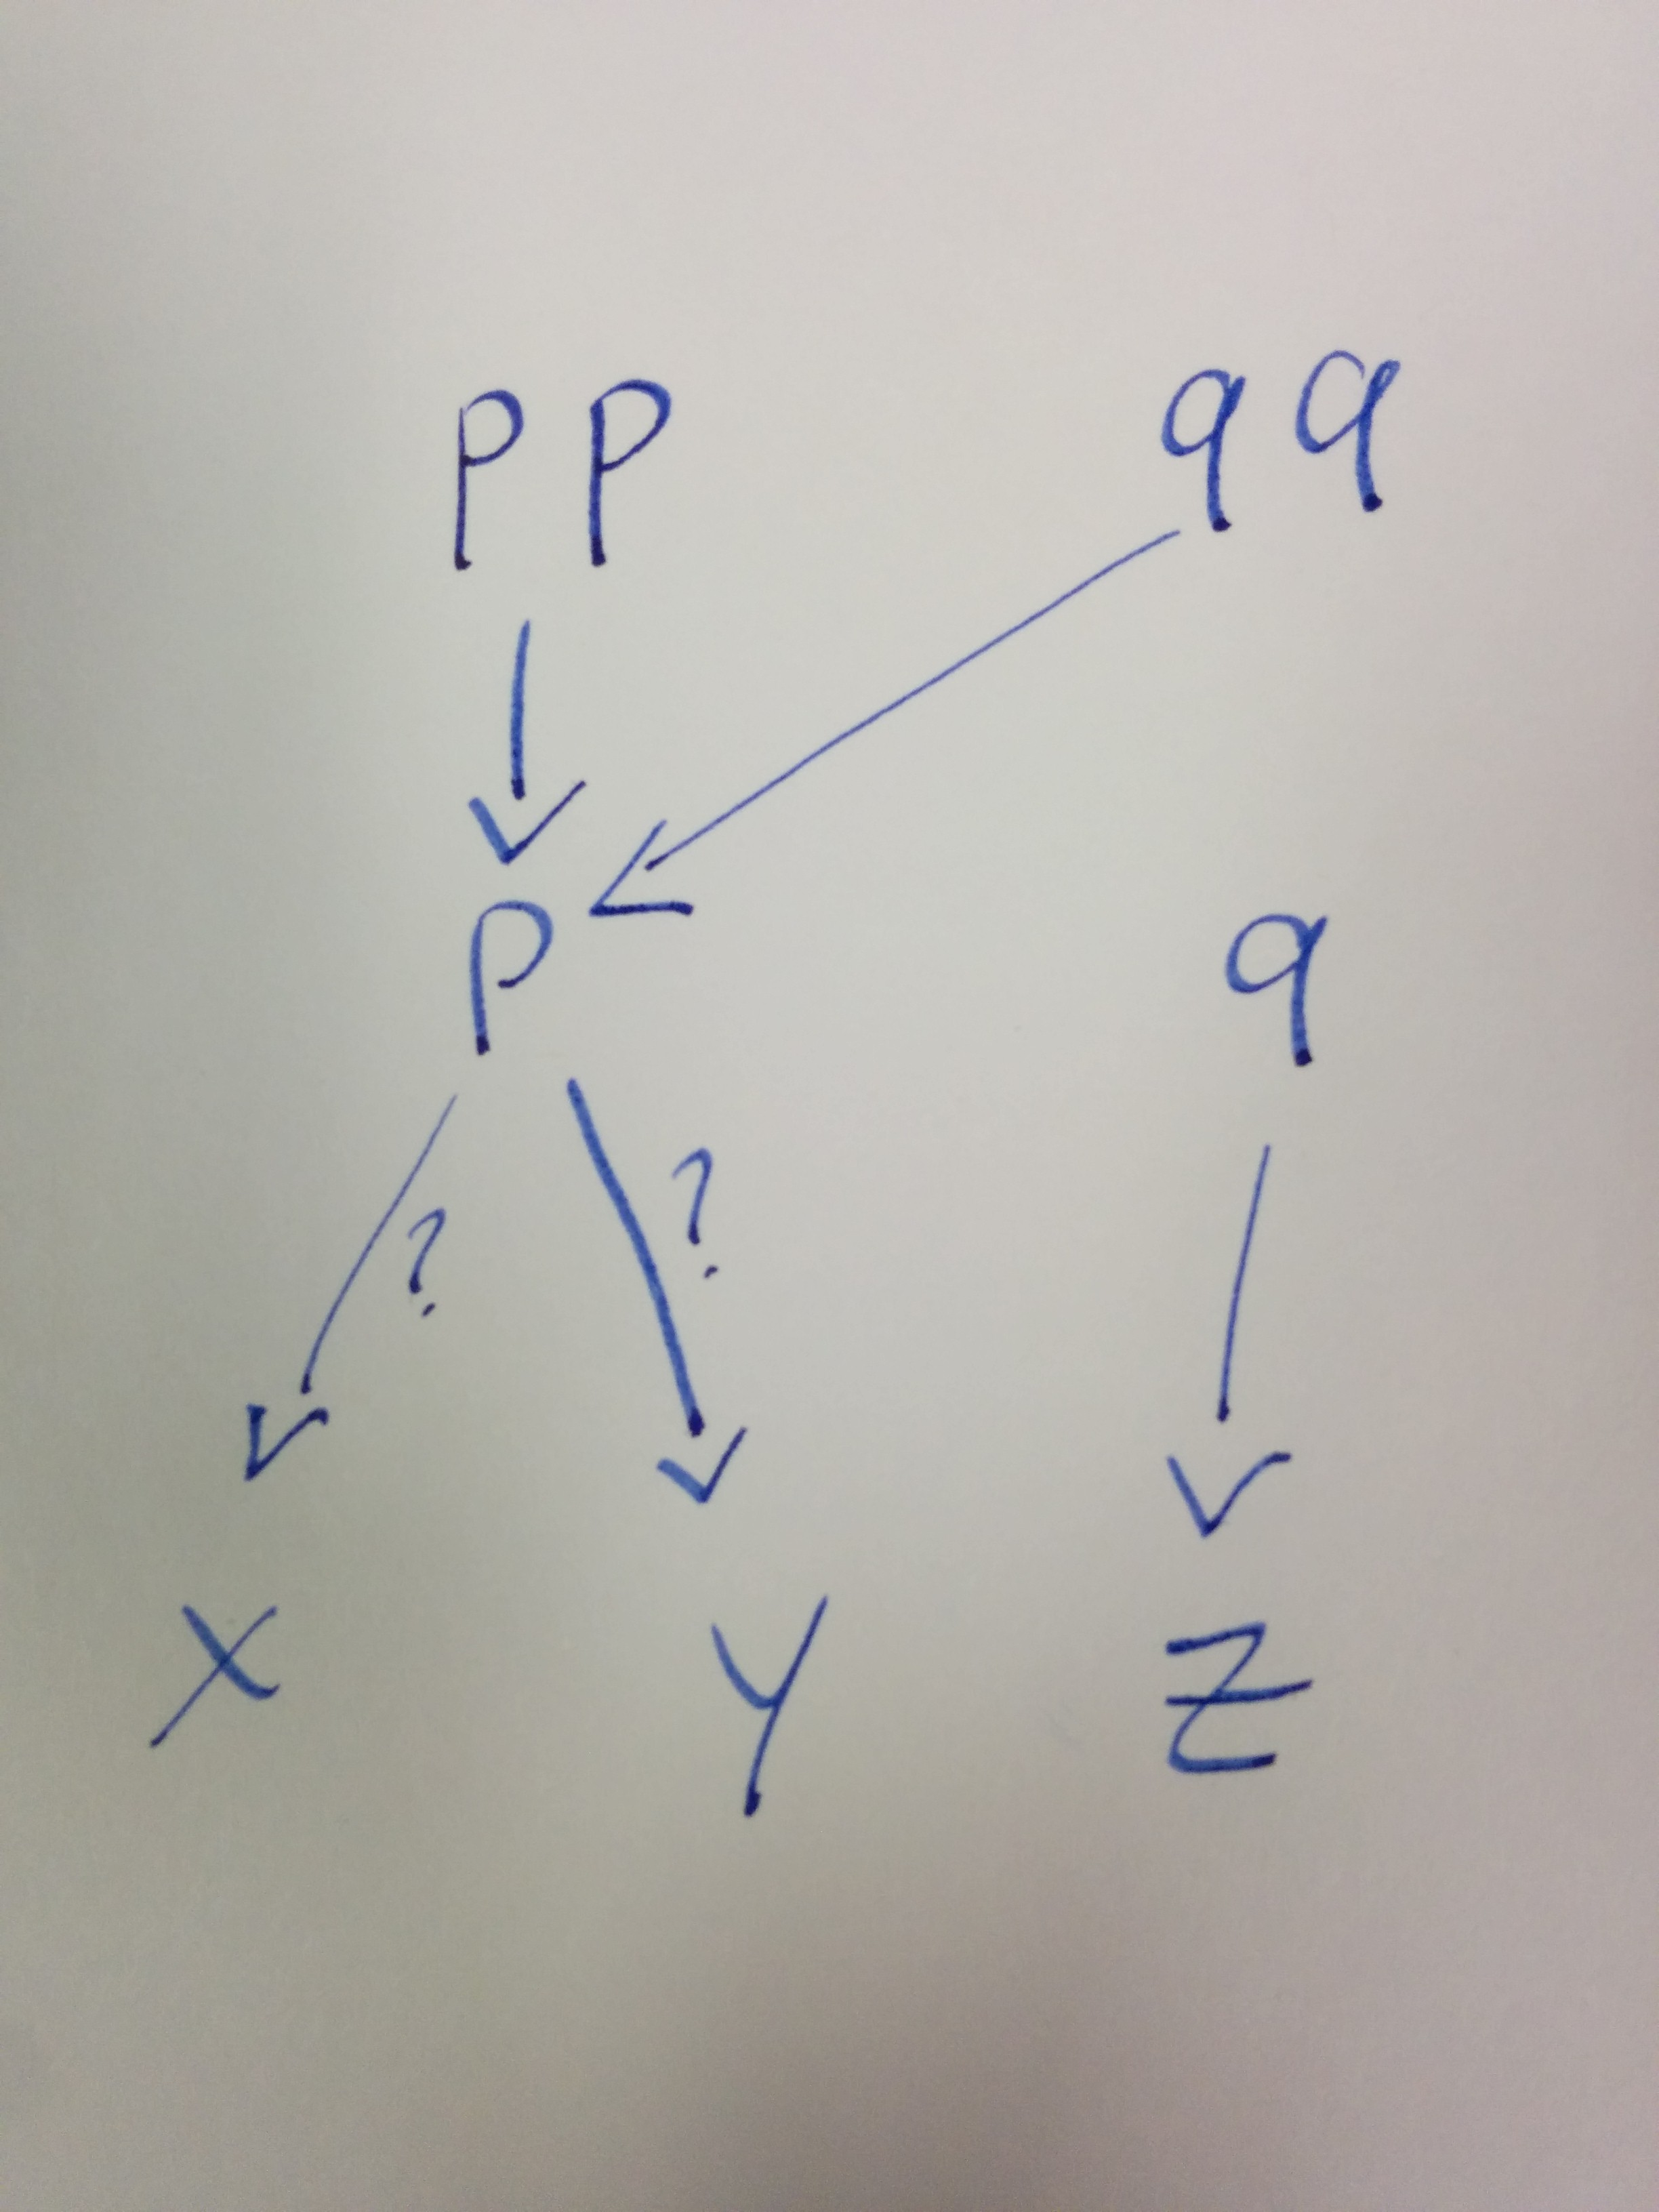
\includegraphics[width=0.2\textwidth]{diagram.jpg}
  \caption{
    The flow-insensitive points-to diagram for the function \codesnip{foo}.
  }
  \label{fig:points-to}
\end{figure}

\section{Stefan's special topic question}

\begin{displayquote}
  \emph{How would you go about garbage collection without any tags?}
\end{displayquote}

It is seen in the presentation that tags are unnecessary for values in
registers, in data structures, or on the stack, but that they are necessary for
heap-allocated data structures. Tags become necessary when representations are
not uniform: if we have a data structure whose representation is unknown, then
a tag can be added so that scrutinizing the tag allows us to know which
representation was used. Tags can therefore be eliminated by using a uniform
representation for heap objects: if everything is represented the same way,
then we already know the layout of the data, which simplifies garbage
collection.

There is an additional complication with this scheme though. An inversion of
control is also necessary to accomplish tag-free garbage collection. It's not
enough to know that data structures are represented uniformly, because data
structures can have variables sizes. Consider a data structure with $n$
components; in principle it must contain $n$ pointers, to refer to those
components. Hence there is no way for a process outside of the data structure
itself to know how many components the data structure contains without
analyzing the data structure, which amounts to a tag analysis. Instead, the
trick is to write the relevant garbage collection routine \emph{into the data
structure} itself. In fact, this is the approch used by GHC, which uniformly
represents heap objects as closures.

In the GHC runtime, each heap object consists of one info pointer (which points
to a statically allocated info table that describes the object) followed by
zero or more pointers to other heap-allocated objects followed by zero or more
unboxed values\footnotemark. The info table is unique up to the (Haskell) type
of the heap object (so it can be shared amongst all runtime values of that
type) and contains pointers to code segments that implement the garbage
collection routine specialized for that data structure. These specialized
routines know the data layout intrinsically and so do not need to analyze any
tags to discover it.

We can see this scheme from another perspective. Suppose there is a general
garbage collection routine takin two parameters: the runtime layout of the heap
object to collect as well as the pointer to that heap object. Since the runtime
layout of each data type is known statically, this general routine can be
partially applied with this static information, and inlined into the generated
object code. This is essentially how the GHC runtime implements its garbage
collection in a tag-free way.

\footnotetext{
  These are values stored directly inside the heap object rather than in
  separate heap objects. Recall that Haskell supports unboxed values, which can
  improve performance in some contexts since indirections are eliminated in the
  representation, but can degrade performance in other contexts since the size
  of the heap object may become unwieldy if the inlined data are themselves
  large.
}

\section{My special topic question}

\begin{enumerate}
  \item
    My special topic question is
    \begin{displayquote}
      Strictness analysis attempts to determine which parameters a function
      will always evaluate. How can strictness analysis be used to optimize a
      function?
    \end{displayquote}

  \item
    Haskell is a non-strict language, meaning that expressions are evaluated on
    a need-to-know basis, and only to the extent that they need to be
    evaluated. The paper I presented discusses the strategies employed by GHC
    to efficiently implement lazy evaluation, but even these tricks have
    overhead. I chose this question because interesting optimization
    opportunities arise when a function is guaranteed to evaluate one or more
    of its parameters.

  \item
    In the presentation, it is seen that all heap objects are uniformly
    represented as closures. However, entering closures is costly because it
    involves executing a jump instruction. Sometimes, closures may also consume
    more space than the data they compute. This is commonly the case for
    arithmetic: the expression \codesnip{let z = x + y} will be represented as
    a suspended computation with two pointers to the free variables
    $x$ and $y$ as well as an additional pointer to the $+$ function. However,
    if we have an expression such as
    \codesnip{case z of 0 -> A ; \textunderscore{} -> B}
    after -- i.e. $z$ is scrutinized -- then the compiler is free
    to eliminate the suspended computation representing $z$ and instead
    immediately compute $z$ at the time that the binding is created. This saves
    space because storing the result of the operation (a mere integer -- $32$
    or $64$ bits) requires much less space than storing the suspended
    computation (three pointers, so $3 \times 32$ or $3 \times 64$ bits).
    Precomputing the value also saves time: immediately executing the code of
    $+$ is faster than constructing a suspended computation and then entering
    it later.

    Furthermore, it is seen in the presentation that the STG language supports
    unboxed values. Whereas boxed values are represented as pointers to
    heap-allocated objects, unboxed values are instead stack-allocated. By
    strictness analysis, it can be determined whether the parameters of a
    function are definitely evaluated, and in those cases, a function accepting
    boxed values can instead be replaced by a function accepting unboxed
    values. (There are some additional considerations regarding polymorphism,
    but this is the correct intuition.) Consequently, its parameters are passed
    via the stack which is significantly faster than requiring the function to
    follow pointers into the heap.

    A correct answer to my question would mention the potential space and time
    savings and justify them with a similar example in which a suspended
    computation is constructed and immediately destructed.
\end{enumerate}

\end{document}
